\chapter{Prácticas Árboles}
En este capítulo encontrarás todas las prácticas sobre los árboles binarios, generales, ABB, entre otros.

\section*{Práctica 1: Árboles Binarios I}
\phantomsection
\addcontentsline{toc}{section}{Práctica 1: Árboles Binarios I}
\label{sec:practica1}
Para poder resolver esta práctica es necesario haber visto el Tema 2: Árboles Binarios (para poder saber cual es la especificación del TAD Abin).

Además vamos a incluir los siguientes ficheros de cabecera:
\begin{minted}[breaklines]{C++}
#include <iostream>
#include "abin_E-S.h"
#include "abin.h" //contiene la especificación e implementación del TAD
\end{minted}

\textbf{\large\underbar{Ejercicio 1:}}\textit{ Implementa un subprograma que calcule el número de nodos de un árbol binario.}

Para calcular el número de nodos de un árbol binario vamos a crear una función recursiva no final, la cual por cada iteración vaya incrementando su valor hasta que termine de recorrer todos los nodos del árbol, hacemos una función llamadora ya que el método \texttt{contarnodos()} solamente recibe el árbol y por tanto necesitamos especificar en que nodo comienza.
\begin{minted}[breaklines]{C++}
template <typename T> size_t contarnodos(const Abin<T>& A){
  //Comprobamos que el árbol no esté vacío
  if(A.raiz() == Abin<T>::NODO_NULO)
    return 0;
  else
    return contarnodos_rec(A.raiz(),A);
}

template <typename T> size_t contarnodos_rec(typename Abin<T>::nodo n, const Abin<T>& A){
  //Caso base
  if(n == Abin<T>::NODO_NULO)
    return 0; //si no hay nodo, devuelve 0
  else
    return 1+contarnodos_rec(A.hijoIzqdo(A),A) + contarnodos_rec(A.hijoDrcho(A),A);
}
\end{minted}

\textbf{\large\underbar{Ejercicio 2:}}\textit{ Implementa un subprograma que calcule la altura de un árbol binario.}

La altura en un árbol es la longitud de la rama más larga, por lo que desde el nodo raíz iremos calculando la longitud de todas las ramas y nos quedaremos con la más grande.

Si el árbol está vacío su altura será -1, si solamente tiene el nodo raíz esta será 0.
\begin{minted}[breaklines]{C++}
template <typename T> size_t alturaAbin(const Abin<T>&A){
    return alturaAbin_rec(A.raiz() , A);
}

template <typename T> size_t alturaAbin_rec(typename Abin<T>::nodo n, const Abin<T>& A){
  //Caso base
  if(n == Abin<T>::NODO_NULO)
    return -1; //un nodo nulo no tiene altura, puesto que indica no existencia de nodo
  else
    return 1+std::max(alturaAbin_rec(A.hijoIzqdo(n),A),
      alturaAbin_rec(A.hijoDrcho(n),A));
}
\end{minted}

\textbf{\large\underbar{Ejercicio 3:}}\textit{ Implementa un subprograma que, dados un árbol binario y un nodo del mismo, determine la profundidad de este nodo en dicho árbol.}

La profundidad es la longitud del único camino desde dicho nodo hasta la raíz del árbol, por tanto, una vez más vamos a implementar una función recursiva que nos calcule la profundidad de dicho nodo.
\begin{minted}[breaklines]{C++}
template <typename T> size_t profundidad_rec(typename Abin<T>::nodo n, const Abin<T>&A){
  if(n == A.raiz()) //la profundidad de la raiz es 0.
    return 0;
  else
    return 1+profundidad_rec(A.padre(n),A);
}
\end{minted}

\textbf{\large\underbar{Ejercicio 4:}}\textit{ Añade dos nuevas operaciones al TAD árbol binario, una que calcule la profundidad de un nodo y otra que calcule la altura de un nodo en un árbol dado. Implementa esta operación para la representación vectorial (índices del padre, hijo izquierdo e hijo derecho).}

Este ejercicio tendremos que incluirlo en el fichero `abin.vec\_1' (las incluimos dentro de la clase y las implemetamos). Como en la implementación vectorial no podemos realizar la llamada mediante la estructura \texttt{celda}, por lo que tendremos que hacer uso del vector de nodos `\texttt{nodos}' para poder acceder al padre e hijos, siendo el acceso al padre (\texttt{nodos[n].padre}), acceso al hijo izquierdo (\texttt{nodos[n].hizq}) y acceso al hijo derecho (\texttt{nodos[n].hder}).

Como estamos dentro del TAD Abin\_vec no hace falta hacer uso del operador de resolución de ámbito `::' para incluir el \texttt{NODO\_NULO} o el nodo en sí.
\begin{minted}[breaklines]{C++}
//Profundidad de un nodo
template <typename T> size_t Abin<T>::profundidad_vec(nodo n){
  //La profundidad de la raiz es 0
  if(n == 0) return 0;
  else
    return 1+profundidad_vec(nodos[n].padre);
}

//Altura del árbol
template <typename T> size_t Abin<T>::altura_vec(nodo n)const{
  //La altura de un nodo nulo no existe, puesto que este indica no existencia de nodo
  if(n == NODO_NULO) return -1;
  else
    return 1+std::max(altura_vec(nodos[n].hizq),altura_vec(nodos[n].hder));
}
\end{minted}

\textbf{\large\underbar{Ejercicio 5:}}\textit{ Repite el ejercicio anterior para la representación enlazada de árboles binarios (punteros al padre, hijo izquierdo e hijo derecho).}

Este ejercicio lo incluiremos en el fichero `abin.h' y ahora el acceso al padre e hijos se realiza mediante punteros, de la forma \texttt{nodo\(\rightarrow\)padre}(acceso al padre), \texttt{nodo\(\rightarrow\)hizq}(acceso al hijo izquierdo) y \texttt{nodo\(\rightarrow\)hder}(acceso al hijo derecho).

Al igual que en el ejercicio 4, no nos hace falta hacer uso del operador de resolución de ámbito, puesto que estamos dentro del contexto del TAD Abin (enlazado).
\begin{minted}[breaklines]{C++}
//Profundidad de un nodo
template <typename T> size_t Abin<T>::profundidad_enla(nodo n){
  //La profundidad de la raiz es 0
  if(n == r) return 0;
  else
    return 1+(profundidad_enla(n->padre));
}

//Altura del árbol
template <typename T> size_t Abin<T>::altura_enla(nodo n){
//La altura de un nodo nulo no existe, puesto que este indica no existencia de nodo
  if(n == NODO_NULO)
    return -1;
  else
    return 1+std::max(altura_enla(n->hizq),altura_enla(n->der));
}

\end{minted}
\textbf{\large\underbar{Ejercicio 6:}}\textit{ Implementa un subprograma que determine el nivel de desequilibrio de un árbol binario, definido como el máximo desequilibrio de todos sus nodos. El desequilibrio de un nodo se define como la diferencia entre las alturas de los subárboles del mismo.}

Como hemos visto en la teoría, el desequilibrio del un árbol es la máxima diferencia de las alturas de los subárboles, por tanto, vamos a implementar una función recursiva que nos lo calcule.

También haremos uso del método altura del ejercicio 2 de esta misma práctica ya que nos ayudará a obtener la altura de cada subárbol.

\begin{minted}[breaklines]{C++}
template <typename T>
size_t desequilibrio(const Abin<T> &A){
    return desequilibrio_rec(A.raiz(), A);
}

template <typename T> size_t desequilibrio_rec(typename Abin<T>::nodo n, const Abin<T> &A){
  if (n == Abin<T>::NODO_NULO)
    return 0;
  else
    return std::max(std::abs(A.alturaAbin_rec(A.hijoIzqdo(n), A) - A.alturaAbin_rec(A.hijoDrcho(n) A)), std::max(desequilibrio_rec(A.hijoIzqdo(n), A), desequilibrio_rec(A.hijoDrcho(n), A)));
}
\end{minted}
\textbf{\large\underbar{Ejercicio 7:}}\textit{ Implementa un subprograma que determine si un árbol binario es o no pseudocompleto.
En este problema entenderemos que un árbol es pseudocompleto, si en el penúltimo nivel
del mismo cada uno de los nodos tiene dos hijos o ninguno.}

Como tenemos que comprobar si tiene o no los dos hijos los nodos del último nivel, vamos a crear una función llamada esHoja la cual nos devolverá un valor booleano dependiendo si el nodo tiene algún nodo o ninguno, en el caso de que tenga al menos uno, devuelve false, de lo contrario devolverá true (no tiene ningún hijo).

Pero también necesitamos una manera de indicar si ese nodo tiene los dos hijos, para ello crearemos otra función llamada dosHijos que devuelve true en el caso de que ese nodo tenga tanto hijo izquierdo, como derecho, en el caso contrario devuelve falso.

Como estamos trabajando con un árbol binario cuya implementación es la enlazada, haremos uso del método que calcula la altura implementado en el ejercicio 5

\begin{minted}[breaklines]{C++}
template <typename T> bool esHoja(typename Abin<T>::nodo n, const Abin<T>& A){
  return (A.hijoIzqdo(n)==Abin<T>::NODO_NULO && A.hijoDrcho(n) == Abin<T>::NODO_NULO);
}

template <typename T> bool dosHijos(typename Abin<T>::nodo n, const Abin<T>& A){
  return (A.hijoIzqdo(n)!=Abin<T>::NODO_NULO && A.hijoDrcho(n)!=Abin<T>::NODO_NULO);
}

template <typename T> bool pseudocompleto(const Abin<T>& A){
  if(A.arbolVacio() || alturaAbin(A) == 0) return true;
  else  return pseudocompleto_rec(A.raiz(), A);
}

template <typename T> bool pseudocompleto_rec(typename Abin<T>::nodo n, const Abin<T>& A){
  if(A.altura_enla(n) == 1)
    return (dosHijos(n,A));
  else{
    if(A.alura_enla(A.hijoIzqdo(n))>A.altura_enla(A.hijoDrcho(n)))
      return pseudocompleto_rec(A.hijoIzqdo(n),A);
    else if(A.alura_enla(A.hijoIzqdo(n))<A.altura_enla(A.hijoDrcho(n)))
      return pseudocompleto_rec(A.hijoDrcho(n),A);
    else  return (pseudocompleto_rec(A.hijoIzqdo(n),A) && pseudocompleto_rec(A.hijoDrcho(n),A));
  }
}
\end{minted}



\newpage
\section*{Práctica 2: Árboles Binarios II}
\phantomsection
\addcontentsline{toc}{section}{Práctica 2: Árboles Binarios II}
\label{sec:practica2}
En esta práctica seguiremos trabajando con los árboles binarios pero resolveremos ejercicios un poco más complejos.

Como fichros de cabecera seguiremos teniendo los mismos que en la práctica 1.

\textbf{\large\underbar{Ejercicio 1:}}\textit{ Dos árboles binarios son similares cuando tienen idéntica estructura de ramificación,
es decir, ambos son vacíos, o en caso contrario, tienen subárboles izquierdo y derecho
similares. Implementa un subprograma que determine si dos árboles binarios son
similares.}

En este ejercicio vamos a realizar una comparación entre dos árboles binario comparando cada subárbol de cada uno para ver si tienen la misma ramificación, por ello vamos a necesitar dos árboles y dos nodos en la función recursiva, la cual devolverá true si ambos árboles tienen la misma ramificación y en el caso contrario devuelve false.

\begin{minted}[breaklines]{C++}
template <typename T> bool similares(const Abin<T>& A, const Abin<T>& B){
  return similares_rec(A.raiz(),B.raiz());
}

template <typename T> bool similares_rec(typename Abin<T>::nodo nA, typename Abin<T>::nodo nB, const Abin<T>& A, const Abin<T>& B){
  if(nA == Abin<T>::NODO_NULO || nb == Abin<T>::NODO_NULO)
    return nA == Abin<T>::NODO_NULO && nb == Abin<T>::NODO_NULO;
  else //Vamos a comprobar la ramificación de sus hijos
    return similares_rec(A.hijoIzqdo(nA), B.hijoIzqdo(nB),A,B) &&
      similares_rec(A.hijoDrcho(nA), B.hijoDrcho(nB),A,B);
}
\end{minted}

\textbf{\large\underbar{Ejercicio 2:}}\textit{ Para un árbol binario \(B\), podemos construir el árbol binario reflejado \(B^R\) cambiando los subárboles izquierdo y derecho en cada nodo. Implementa un subprograma que devuelva el árbol binario reflejado de uno dado.}

\begin{minted}[breaklines]{C++}
//Declaración adelanta del método reflejado_rec
template <typename T> void reflejado_rec(typename Abin<T>::nodo nA, typename Abin<T>::nodo nB,const Abin<T>& A, Abin<T>& B);

template <typename T> Abin<T> reflejado (const Abin<T> A){
  //Creamos el árbol binario a devolver
  Abin<T> B;
  if(!A.arbolVacio()){
    B.insertarRaiz(A.elemento(A.raiz())); //inicializamos el árbol B con la raiz de A
    reflejado_rec(A.raiz(),B.raiz(),A,B);
  }
  return B; //Devolvemos el árbol reflejado
}
template <typename T> void reflejado_rec(typename Abin<T>::nodo nA, typename Abin<T>::nodo nB,const Abin<T>& A, Abin<T>& B){
  //Comprobamos caso base, que el nodo nA no sea nulo
  if(nA!=Abin<T>::NODO_NULO){
    if(A.hijoIzqdo(nA)!=Abin<T>::NODO_NULO){ //Si A tiene Hizqdo, se inserta en Hder de B
      B.insertarHijoDrcho(nB,A.elemento(A.hijoIzqdo(nA)));
      reflejado_rec(A.hijoIzqdo(nA),nB,A,B);
    }
    if(A.hijoDrcho(nA)!= Abin<T>::NODO_NULO){//Si A tiene Hder, se inserta en Hizq de B
      B.insertarHijoIzqdo(nB,A.hijoDrcho(nA),A,B);
      reflejado_rec(A.hijoDrcho(nA),nB,A,B);
    }
    //Si los hijos de nA son hoja, no hace nada.
  }
  //Si nA es hoja, no hace nada.
}
\end{minted}
\textbf{\large\underbar{Ejercicio 3:}}\textit{ El TAD árbol binario puede albergar expresiones matemáticas mediante un árbol de expresión. Dentro del árbol binario los nodos hojas contendrán los operandos, y el resto de los nodos los operadores.}
\begin{enumerate}[label=\alph*)]
  \item Define el tipo de los elementos del árbol para que los nodos puedan almacenar
  operadores y operandos.
  \item Implementa una función que tome un árbol binario de expresión (aritmética) y
  devuelva el resultado de la misma. Por simplificar el problema se puede asumir que el
  árbol representa una expresión correcta. Los operadores binarios posibles en la expresión
  aritmética serán suma, resta, multiplicación y división.
\end{enumerate}
Sea la operación aritmética \(\rightarrow\) \textbf{7×(15 - 3,2)/2}
\begin{figure}[h]
  \begin{center}
    \includegraphics*[width=.3\textwidth]{assets/p2.1.png}
  \end{center}
  \caption{Ejemplo árbol binario de expresión (aritmética)}
\end{figure}

\underbar{Nota:} En el programa de prueba podemos usar las funciones rellenarAbin() de abin\_E-S.h para introducir por teclado o desde un fichero el árbol de expresión a evaluar. Sin
embargo, en este caso, será necesario sobrecargar los operadores utilizados internamente
en dichas funciones, es decir \(>>\), \(<<\) y \(!=\) para el tipo de los elementos del árbol.

Como vemos en la \textit{Figura 1.1} los nodos que no son hojas son los que contienen los operadores aritméticos. Para poder introducir un número este nodo tiene que ser hoja por eso vamos a hacer uso de la función \texttt{esHoja()}.
\begin{minted}[breaklines]{C++}
template <typename T> bool esHoja(typename Abin<T>::nodo n, const Abin<T>& A){
  return (A.hijoIzqdo(n) == Abin<T>::NODO_NULO && A.hijoDrcho(n)==Abin<T>::NODO_NULO);
} 
\end{minted}

Vamos a crear un tipo \texttt{Enum} que va a contener los operadores aritméticos.
\begin{minted}[breaklines]{C++}
enum operador{suma = '+', resta = '-', producto = '*', division = '/'};
\end{minted}

Como vemos en el ejemplo del enunciado una expresión es la unión de un número con su operador
\begin{minted}[breaklines]{C++}
union expresion{
  double num;
  operador op;};
\end{minted}

Como ya tenemos todos los componentes del ejercicio declarados, vamos a implementar la función que nos calcula la expresión aritmética.
\begin{minted}[breaklines]{C++}
double calcular(const Abin<expresion>& A){
  return calcular_rec(A.raiz(),A);
}

double calcular_rec(typename Abin<expresion>::nodo n, const Abin<expresion>& A){
  //Si el nodo es hoja, es el contenido del nodo es un número
  if(esHoja(n,A)){
    return A.elemento(n).num;
  }
  else{ //es un operador aritmético
    switch(A.elemento(n).op){
      case suma:
        return calcular_rec(A.hijoIzqdo(n),A) + calcular_rec(A.hijoDrcho(n),A);
        break;
      case resta:
        return calcular_rec(A.hijoIzqdo(n),A) - calcular_rec(A.hijoDrcho(n),A);
        break;
      case producto:
        return calcular_rec(A.hijoIzqdo(n),A) * calcular_rec(A.hijoDrcho(n),A);
        break;
      case division:
        return calcular_rec(A.hijoIzqdo(n),A) / calcular_rec(A.hijoDrcho(n),A);
        break;
    }
  }
}
\end{minted}
% \textbf{\large\underbar{Ejercicio 4:} }

\newpage
\section*{Práctica 3: Árboles Generales}
\phantomsection
\addcontentsline{toc}{section}{Práctica 3: Árboles Generales}
\label{sec:practica3}
En esta práctica vamos a ver como trabajar con el TAD Agen con sus dos representaciones (enlazada y vectorial).

Como cabeceras de la práctica vamos a tener:
\begin{minted}[breaklines]{C++}
  #include <iostream>
  #include "agen.h" //Especificación e implementación de los métodos del TAD.
  #include "agen_E-S.h"
\end{minted}

\textbf{\large\underbar{Ejercicio 1:}}\textit{ Implementa un subprograma que dado un árbol general nos calcule su grado.}

Para saber cual es el grado de un árbol este es el máximo de los grados de los nodos que componen al árbol.
Por tanto, para saber cuales el grado del Agen, tenemos que saber cual es el grado de cada nodo que lo compone y quedarnos con el máximo.

\begin{minted}[breaklines]{C++}
template <typename T> size_t gradoAgen(const Agen<T> &A){
  return gradoAgen_rec(A.raiz(),A);
}
template <typename T> size_t gradoAgen_rec(typename Agen<T>::nodo n, const Agen<T> &A){
  if(n == Agen<T>::NODO_NULO){
    return 0; //el grado de un nodo nulo (no existe nodo) es 0
  }
  else{
    size_t gradoMax = 0; //grado del árbol
    size_t nHijos = 0; //grado del nodo
    typename Agen<T>::nodo aux = A.hijoIzqdo(n);
    //Calculamos el grado del árbol.
    while(aux != Agen<T>::NODO_NULO){
      nHijos++;
      gradoMax = std::max(gradoMax,gradoAgen_rec(aux,A));
      aux = A.hermDrcho(aux);
    }
    return std::max(nHijos,gradoMax);
  }
}
\end{minted}

\textbf{\large\underbar{Ejercicio 2:}}\textit{ Implementa un subprograma que dados un árbol y un nodo dentro de dicho árbol determine la profundidad de éste nodo en el árbol.}

Para calcular la profundidad de un nodo cualquiera en un árbol general, este se va a calcular de la misma forma que en los árboles binarios, ya que lo que tenemos que hacer es partir del nodo en cuestión e ir llamando al padre del mismo hasta llegar a la raiz.

\begin{minted}[breaklines]{C++}
template <typename T> size_t profundidadAgen_rec(typename Agen<T>::nodo n, const Agen<T> &A){
  if(n == A.raiz())
    return 0;
  else
    return 1+profundidadAgen_rec(A.padre(n),A);
}
\end{minted}

\textbf{\large\underbar{Ejercicio 3:}}\textit{ Se define el desequilibrio de un árbol general como la máxima diferencia entre las alturas de los subárboles más bajo y más alto de cada nivel. Implementa un subprograma que calcule el grado de desequilibrio de un árbol general.}

Vamos a suponer que tenemos un método llamado \texttt{alturaAgen()}, el cual nos hará falta para poder calcular el desequilibrio de un árbol general (según la definició de desequilibrio dada).

Para calcular el desequilibrio vamos a recorrer todos los hermanos del hijo del nodo dado, y vamos calculando el desequilibrio máximo mediante la función \texttt{std::max()}.

\begin{minted}[breaklines]{C++}
template <typename T> size_t desequilibrioAgen(const Agen<T> &A){
  return profundidadAgen_rec(A.raiz(),A);
}

template <typename T> size_t desequilibrioAgen_rec(typename Agen<T>::nodo n, const Agen<T> &A){
  if(n == Agen<T>::NODO_NULO){
    return 0;
  }
  else{
    size_t maxDesequilibrio = 0;
    typename Agen<T>::nodo aux = A.hijoIzqdo(n);
    while (aux != Agen<T>::NODO_NULO){
      maxDesequilibrio = std::max(maxDesequilibrio, std::abs(alturaAgen_rec(aux,A) - alturaAgen(A.hermDrcho(aux),A)));

      aux = A.hermDrcho(aux);
    }
    return maxDesequilibrio;
  }
}
\end{minted}

\textbf{\large\underbar{Ejercicio 4:}}\textit{ Dado un árbol general de enteros A y un entero x, implementa un subprograma que realice la poda de A a partir de x. Se asume que no hay elementos repetidos en A.}

Una poda significa que apartir de dicho nodo tenemos que eliminar todos sus desecendientes y a él mismo.

Para ello, primero tenemos que realizar la búsqueda del elemento `x' en el Agen y a partir de su posición eliminar todos los desecendientes.

\begin{minted}[breaklines]{C++}
//Método buscar un nodo a partir de su contenido
template <typename T> typename Agen<T>::nodo buscar(T e, Agen<T> &A){
  return buscar_rec(e,A.raiz(),A);
}
template <typename T> typename Agen<T>::nodo buscar_rec(T e, typename Agen<T>::nodo n, Agen<T> &A){
  if(n==Agen<T>::NODO_NULO){
    return Agen<T>::NODO_NULO;
  }
  else if(A.elemento(n) == e){ //Lo hemos encontrado, lo devolvemos
    return n;
  }
  else{
    //Vamos a buscar en sus hermanos
    typename Agen<T>::nodo aux = A.hijoIzqdo(n);
    while(aux != Agen<T>::NODO_NULO){
      typename Agen<T>::nodo aux2 = buscar_rec(e,aux,A);
      if(aux2 != Agen<T>::NODO_NULO){
        return aux2;
      }
      aux = A.hermDrcho(aux);

    }
    return Agen<T>::NODO_NULO; //no existe entre los hermanos
  }
}

template <typename T> void podaAgen(T x, Agen<T> &A){
  typename Agen<T>::nodo n = buscar(x,A);
  return podaAgen_rec(n,A);
}

template <typename T> void podaAgen_rec(typename Agen<T>::nodo n, Agen<T>: &A){
  if(n != Agen<T>::NODO_NULO){
    //Mientras que n tenga hijos, podamos
    while(A.hijoIzqdo(n)!= Agen<T>::NODO_NULO){
      //Realizamos la llamada recursiva con el hijo (poda del subárbol del hijo)
      podaAgen_rec(A.hijoIzqdo(n),A);
      A.eliminarHijoIzqdo(n); //eliminamos al propio hijo
    }
  }
}
\end{minted}


\newpage
\section*{Práctica 4: Árboles Binarios de Búsqueda}
\phantomsection
\addcontentsline{toc}{section}{Práctica 4: Árboles Binarios de Búsqueda}
\label{sec:practica4}
En esta práctica, veremos como trabajar con árboles binarios de búsqueda (ABB).

A diferencia de los árboles binarios o generales ahora no trabajamos con nodos, si no con subárboles del mismo.

Como ficheros de cabeceras tendremos:
\begin{minted}[breaklines]{C++}
  #include <iostream>
  #include "abb.h" //contiene Especificación e implementación métodos del TAD.
  #include <vector> //para algunos ejercicios
\end{minted}

\textbf{\large\underbar{Ejercicio 1:}}\textit{ Implementa una nueva operación del TAD Abb que tomando un elemento del mismo elimine al completo el subárbol que cuelga de él.}
\underbar{Ejemplo:} Para el árbol binario de búsqueda de la figura se muestra la transformación si la entrada fuera el valor 9.
\begin{figure}[h]
  \begin{center}
    \includegraphics*[width=.7\textwidth]{assets/Abb1.png}
  \end{center}
\end{figure}

Suponemos que estamos dentro del TAD -> `abb.h'
\begin{minted}[breaklines]{C++}
template <typename T> void deletSubarbol(Abb<T> A, const T& e){
  return deletSubarbol_rec(A.r, e);
}

template typename<T> void deletSubarbol_rec(typename Abb<T>::arbol *&a, const T& e){
  if(a != nullptr){
    if( e < a->elto){
      deletSubarbol_rec(a->izq.r,e);
    }
    else if(e > a->elto){
      deletSubarbol_rec (a->der.r, e);
    }
    else{
      delete a;
      a = nullptr;
    }
  }
}
\end{minted}
\newpage
\textbf{\large\underbar{Ejercicio 2:}}\textit{ Un árbol binario de búsqueda se puede equilibrar realizando el recorrido en inorden del árbol para obtener el listado ordenado de sus elementos y a continuación, repartir equitativamente los elementos a izquierda y derecha colocando la mediana en la raíz y construyendo recursivamente los subárboles izquierdo y derecho de cada nodo. Implementa este algoritmo para equilibrar un ABB.}

Para llevar a cabo este problema necesitamos almacenar todos los elementos de un Abb y mediante un recorrido en inorden realizar la inserción de dicho elementos de menera equitativa con el fin de obtener un ABB equilibrado. Aquí está el motivo de porque incluimos la cabecera \texttt{<vector>}.

Además vamos a construir el árbol equilibrado a partir del vector con los elementos, por eso el método \texttt{equilibrarABB\_rec()} recibe dos enteros; posición inicio y fin del vector.

A partir de ahí se calcula la mediana que concuerda con el elemento que será la raiz del ABB.

\begin{minted}[breaklines]{C++}
template <typename T> void equilibrarABB(Abb<T> &A){
//Creamos el vector que contendrá los elementos del ABB
  vector<T> v;
//Recorrido en inorden
  inorden(A, v);
//Equilibramos todo el árbol.
  A.r = equilibrarABB_rec(v,0,v.size()-1);
}

template <typename T> Abb<T>::arbol* equilibrarABB_rec(std::vector<T> &v, size_t ini, size_t fin){
  if(ini > fin){
    return nullptr;
  }
  else{
    //sacamos la raiz
    size_t mediana = (ini+fin)/2;
    //creamos un nuevo árbol con el valor de la mediana como raiz
    typename Abb<T>::arbol* a = new typename Abb<T>::arbol(v[mediana]);
    //insertamos los elementos de forma equitativa
    a->izq.r = equilibrarABB_rec(v, ini,mediana-1);
    a->der.r = equilibrarABB_rec(v,mediana+1,fin);
    return a; //devolvemos el árbol equilibrado
  }
}
\end{minted}

\textbf{\large\underbar{Ejercicio 3:}}\textit{ Dados dos conjuntos representados mediante árboles binarios de búsqueda, implementa la operación unión de dos conjuntos que devuelva como resultado otro conjunto que sea la unión de ambos, representado por un ABB equilibrado.}


\begin{minted}[breaklines]{C++}
template <typename T> Abb<T> Union(const Abb<T> &A, Abb<T>B){
  //Declaramos un Abb con el contenido de A que será el resultado de la unión de A y B.
  Abb<T> Res{A}; 
  while(!B.vacio()){
    //Insertamos los elemento que no se encuentren en A
    if(A.buscar(B.elemento()).vacio()){
      Res.insertar(B.elemento());
    }
    B.eliminar(B.elemento());
  }
  Equilibrar(Res);
  return Res;
}
\end{minted}

\textbf{\large\underbar{Ejercicio 4:}}\textit{ Dados dos conjuntos representados mediante árboles binarios de búsqueda, implementa la operación intersección de dos conjuntos, que devuelva como resultado otro conjunto que sea la intersección de ambos. El resultado debe quedar en un árbol equilibrado.}
\begin{minted}[breaklines]{C++}
template <typename T> Abb<T> Intersec(const Abb<T> &A, Abb<T> B){
  //Declaramos un Abb vacio que será el resultado de la unión de A y B.
  Abb<T> Res;
  while(!B.vacio()){
    //insertamos los elementos que se encuentren en A
    if(!A.buscar(B.elemento()).vacio()){
      Res.insertar(B.elemento());
    }
    B.eliminar(B.elemento());
  }
  Equilibrar(Res);
  return Res;
}
\end{minted}

\textbf{\large\underbar{Ejercicio 5:}}\textit{ Implementa el operador $\diamond$ para conjuntos definido como $A \diamond\ B = (A \cup B) - (A \cap B)$. La implementación del operador $\diamond$ debe realizarse utilizando obligatoriamente la operación $\in$, que nos indica si un elemento dado pertenece o no a un conjunto. La representación del tipo Conjunto debe ser tal que la operación de pertenencia esté en el caso promedio en $O(\log n)$.}

Para poder llevar a cabo este subprograma vamos a hacer uso de las dos funciones previamente implementadas (Unión e Intersección) de Abb.
\begin{minted}[breaklines]{C++}
//vamos a crearnos una función auxiliar que nos va a servir de ayuda para comprobar si un elemento existe o no en un conjunto.
template <typename T> bool existe(const T& e, const Abb<T> &A){
  return !A.buscar(e).vacio();
}
template <typename T> Abb<T> opRombo(const Abb<T> &A, Abb<T> B){
  //realizamos la unión e intersección de los árboles
  Abb<T> Union{Union(A,B)};
  Abb<T> Inserseccion{Intersec(A,B)};
  Abb<T> Diff{Union};

  while(!Intersección.vacio()){
    //Si encontramos el elemento en la intersección de A y B, se quita de la diferencia
    if(exite(Interseccion.elemento(),Union)){
      Diff.eliminar(Interseccion.elemento());
    }
    //Si no está, se elimina de la intersección
    Interseccion.eliminar(Interseccion.elemento());
    //Equilibramos el árbol despues de eliminar un elemento.
    Equilibrar(Interseccion);
  }
  //Equilibramos el árbol diferencia "Diff" ya que hemos eliminado del mismo.
  Equilibrar(Diff);
  return Diff;
}
\end{minted}

\newpage
\section*{Práctica 5: Árboles parcialmente ordenados y otros}
\phantomsection
\addcontentsline{toc}{section}{Práctica 5: Árboles parcialmente ordenados y otros}
\label{sec:practica5}

En esta práctica trabajaremos con árboles parcialmente ordenados (APOs o montículos), con árboles B y con otros árboles vistos en prácticas anteriores.

Para poder realizar esta práctica vamos a poner como ficheros de cabeceras:
\begin{minted}[breaklines]{C++}
  #include <iostream>
  #include "abin.h"
  #include "agen.h"
  #include <vector> //para algunos ejercicios
  #include <string.h> //para algunso ejercicios
\end{minted}

\textbf{\large\underbar{Ejercicio 1:}}\textit{ Dado un árbol binario de enteros donde el valor de cada nodo es menor que el de sus hijos, implementa un subprograma para eliminar un valor del mismo preservando la propiedad de orden establecida. Explica razonadamente la elección de la estructura de datos.}

\underbar{Nota:} Se supone que en el árbol no hay elementos repetidos, y que el número de nodos del mismo no está acotado.

Según el enunciado tenemos un Abin que se comporta como un ABB debido a que el valor de los nodos que son descendientes son mayores que el del padre.
Además si queremos que al eliminar cualquier nodo el árbol siga cumpliendo la propiedad de orden y sabiendo que no podemos eliminar un nodo que no sea hoja, tendremos que intercambiarlo por el nodo cuyo valor sea el menor de los dos hasta que el nodo a eliminar sea una hoja.

Por tanto, nuestra función tendrá como parámetros de entrada el elemento del nodo (para poder buscarlo), el nodo (para poder trabajar con él) y el árbol.
\begin{minted}[breaklines]{C++}
//Métodos auxiliares
template <typename T> bool dosHijos(typename Abin<T>::nodo n, Abin<T> &A){
  return (A.hijoIzqdo(n)!=Abin<T>::NODO_NULO && A.hijoDrcho(n)!=Abin<T>::NODO_NULO);
}

template <typename T> bool esHoja (typename Abin<T>::nodo n, const Abin<T> &A){
  return (A.hijoIzqdo(n) == Abin<T>::NODO_NULO && A.hijoDrcho(n) == Abin<T>::NODO_NULO);
}

template <typename T> Abin<T>::nodo minimo (typename Abin<T>::nodo a,typename Abin<T>::nodo a const Abin<T> &A){
  if(a == Abin<T>::NODO_NULO) return b;
  if(b == Abin<T>::NODO_NULO) return a;
  else return (A.elemento(a) < A.elemento(b)) ? a : b;
}

template <typename T> void eliminar (const T& e, const Abin<T> &A){
  eliminar_rec(e, A.raiz(), A);
}
template <typename T> void eliminar_rec(const T& e, typename Abin<T>::nodo n, Abin<T> &A){
  if(n != Abin<T>::NODO_NULO){
    //Buscamos el nodo que tenga ese elemento
    if(A.elemento(n) == e){
      if(!esHoja(n,A)){
        //Si no es una hoja puede tener 1 ó 2 hijos
        if(dosHijos(n,A)){
          //Si tiene ambos hijos, intercambiamos con el menor de los 2 y el otro pasa a ser hijo
          typename Abin<T>::nodo hijo = minimo(A.hijoIzqdo(n),A.hijoDrcho(n),A);
          A.elemento(n) = A.elemento(hijo);
          eliminar_rec(A.elemento(hijo),hijo,A); //seguimos bajando
        }
        else{ //tiene 1 (puede ser el izquierdo o derecho)
          typename Abin<T>::nodo hijo = (A.hijoIzqdo(n) != Abin<T>::NODO_NULO) ? A.hijoIzqdo(n) : A.hijoDrcho(n);
          A.elemento(n) = A.elemento(hijo);
          eliminar_rec(A.elemento(hijo),hijo,A); //seguimos bajando
        }
      }
      else{
        //es hoja, eliminamos el Nodo
        typename Abin<T>::nodo padre = A.padre(n);
        if (A.hijoIzqdo(padre) == n) {
            A.eliminarHijoIzqdo(padre);
        } else {
            A.eliminarHijoDrcho(padre);
        }
      }
      }else {
        // Seguir buscando en los hijos
        eliminar_rec(e, A.hijoIzqdo(n), A);
        eliminar_rec(e, A.hijoDrcho(n), A);
      }
    //Si es nulo, no hace nada
  }
}

\end{minted}

\textbf{\large\underbar{Ejercicio 2:}}\textit{ Un montículo min-max tiene una estructura similar a la de un montículo ordinario (árbol parcialmente ordenado), pero la ordenación parcial consiste en que los elementos que se encuentran en un nivel par (0, 2, 4,..) son menores o iguales que sus elementos descendientes, mientras que los elementos que se encuentran en un nivel impar (1, 3, 5,..) son mayores o iguales que sus descendientes. Esto quiere decir que para cualquier elemento e de un nivel par se cumple abuelo \(\leq\) e \(\leq\) padre y para cualquier elemento e de un nivel impar padre \(\leq\) e \(\leq\) abuelo.\\
Implementa una operación de orden logarítmico para añadir un elemento a un montículo min-max almacenado en un vector de posiciones relativas.}

Vamos a insertar ese elemento al final del APO, y lo iremos flotando hasta que se quede en la posición correta, por tanto tendremos que realizar una modificación en la función \texttt{flotar()}, ya que como hemos dicho antes, insertarémos por el final del APO.

\begin{minted}[breaklines]{C++}
template <typename T> void APOmM<T>::insertar(const T& e){
  assert(ultimo < maxNodos-1); //APOMinMax no lleno
  nodos[++ultimo] = e; //insertarmos al final e incrementamos el númoero de elementos.
  if(ultimo > 0)
    flotar(ultimo); //reordenamos el APO.
}

template <typename T> void APOmM<T>::flotar(nodo i){
  size_t profundidad = log2(i+1);
  T e = nodos[i];
  T aux;
  nodo abuelo;
  //como i no es raiz, tiene padre
  if(profundidad % 2 == 0){//nivel par
    if(nodos[padre(i)] < nodos[i]){ //Tenemos que reordenar respecto a los niveles impares
      Intercambio(nodos[i],nodos[padre(i)]);
      i = padre(i);
      profundidad--;
      abuelo = padre(padre(i));
      while(abuelo >= 0 && nodos[abuelo] < nodos[i]){
        Intercambio(nodos[i],nodos[abuelo]);
        i = abuelo;
        abuelo = padre(padre(i));
        profundidad-=2;
      }
    }
    else{ //Comprobamos si tenemos que reordenar respecto a los niveles pares del APO.
      abuelo = padre(padre(i));
      while(abuelo >= 0 && nodos[abuelo] > nodos[i]){
        Intercambio(nodos[abuelo],nodos[i]);
        i = abuelo;
        abuelo = padre(padre(i));
        profundidad-=2;
      }
    }
  }else{//nivel impar
    if(padre(i) >= 0 && nodos[padre(i)] > nodos[i]){//Tenemos que reordenar respecto a los niveles pares
      Intercambio(nodos[i],nodos[padre(i)]);
        i = padre(i);
        profundidad--;
        abuelo = padre(padre(i));
        while(abuelo >= 0 && nodos[abuelo] > nodos[i]){
          Intercambio(nodos[i],nodos[abuelo]);
          i = abuelo;
          abuelo = padre(padre(i));
          profundidad-=2;
        }
    }
    else{//Comprobamos si tenemos que reordenar respecto a los niveles pares del APO.
      abuelo = padre(padre(i));
      while(abuelo >= 0 && nodos[abuelo] < nodos[i]){//Reordenamos respecto niveles pares
        Intercambio(nodos[abuelo], nodos[i]);
        i = abuelo;
        abuelo = padre(padre(i));
        profundidad-=2;
      }
    }
  }
}
\end{minted}

\textbf{\large\underbar{Ejercicio 3:}}\textit{ Implementa una operación de orden logarítmico para eliminar el elemento máximo de un montículo min-max definido como en el problema anterior.}

\begin{minted}[breaklines]{C++}
template <typename T> void APOmM::suprimirMax(){
  assert(ultimo > -1);
  if(--ultimo > -1){//APO no queda vacío
    if(ultimo >= 2){//Tiene dos hijos y al menos 1 nieto, el máximo está en uno de los 2 hijos.
      if(nodos[1] > nodos[2]){
        nodos[1] = nodos[ultimo+1];
        hundir(1);
      }else{
        nodos[2] = nodo[ultimo+1];
        hundir(2);
      }
    }else if(ultimo == 1){
      nodos[1] == std::min(nodos[1],nodos[2])M
    }
  }
}
\end{minted}

\textbf{\large\underbar{Ejercicio 4:}}\textit{ Un árbol es estrictamente ternario si todos sus nodos son hojas o tienen tres hijos. Escribe una función que, dado un árbol de grado arbitrario, nos indique si es o no estrictamente ternario.}

Vamos a partir de un Agen, ya que son los únicos que pueden tener más de dos hijos (un hijo izquierdo y los hermanos de este).

\begin{minted}[breaklines]{C++}
template <typename T> bool esTernario(const Agen<T> &A){
  return esTernario_rec(A.raiz(), A);
}

template <typename T> bool esTernario_rec(typename Agen<T>::nodo n, const Agen<T> &A){
  //n es un nodo nulo
  if(n == Agen<T>::NODO_NULO)
    return true;
  //n no tiene hijos.
  else if(A.hijoIzqdo(n) == Agen<T>::NODO_NULO && A.hermDrcho(n)== Agen<T>::NODO_NULO)
    return true;
  //n tiene hijos
  else if(A.hijoIzqdo(n) != Agen<T>::NODO_NULO && A.hermDrcho(n)!= Agen<T>::NODO_NULO){
    //llamamos a la función para sus hijos
    esTernario_rec(A.hijoIzqdo(n),A) && esTernario_rec(A.hermDrcho(n),A);
  }
  else //Tiene 1 hijo.
    return false;
}
\end{minted}

\textbf{\large\underbar{Ejercicio 5:}}\textit{ Una forma de representar una figura plana en blanco y negro consiste en utilizar un árbol cuaternario en el que cada nodo o tiene exactamente cuatro hijos, o bien es una hoja. Un nodo hoja puede ser blanco o negro y un nodo interno no tiene color.}

Una figura dibujada dentro de un cuadrado de lado 2k se representa de la forma siguiente: Se divide el cuadrado en cuatro cuadrantes y cada uno se representa como un hijo del nodo raíz. Si un cuadrante está completamente negro corresponde a una hoja negra; si, por el contrario, el cuadrante está completamente blanco, éste corresponde a una hoja blanca; y si un cuadrante está parcialmente ocupado por negro y blanco, entonces corresponde a un nodo interno del árbol y este cuadrante se representa siguiendo el mismo método subdividiéndolo en otros cuatro cuadrantes. Como ejemplo se muestra una figura en blanco y negro y su árbol asociado, tomando los cuadrantes en el sentido de las agujas del reloj a partir del cuadrante superior izquierdo.
\begin{figure}[h]
  \begin{center}
    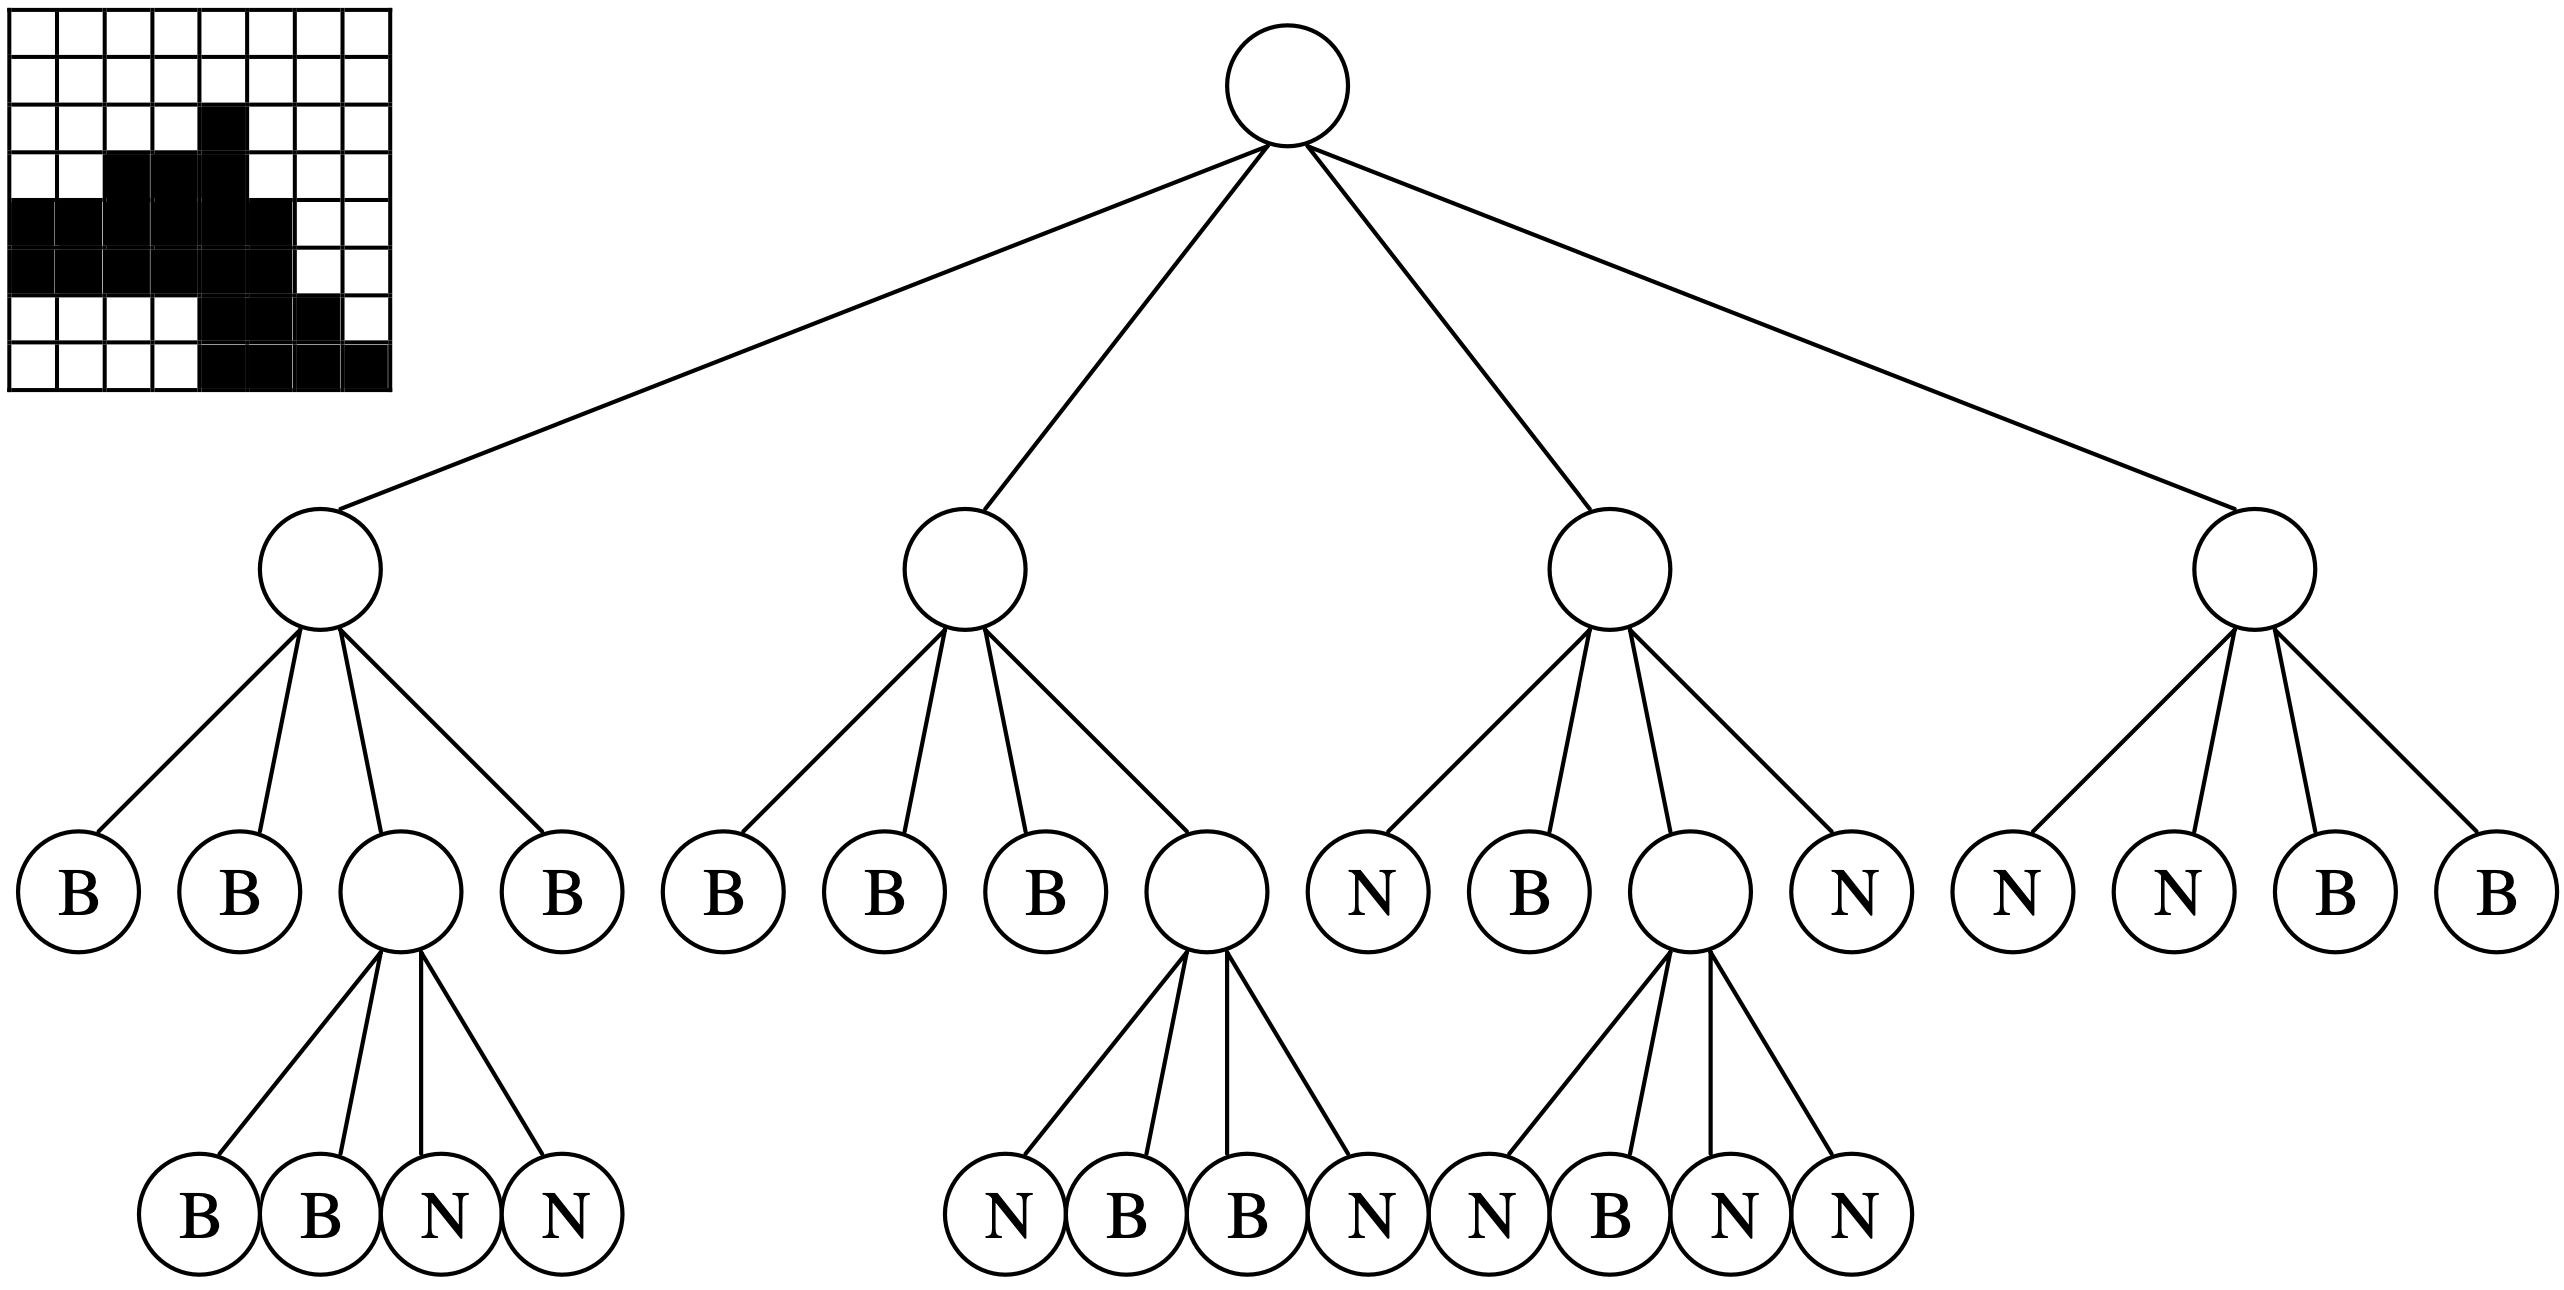
\includegraphics[width=.7\textwidth]{assets/p5.png}
  \end{center}
\end{figure}

Implementa una función que dado un árbol de esta clase, con k+1 niveles, devuelva la figura asociada, representada como una matriz cuadrada de tamaño 2k en la que cada celda representa un punto blanco o negro.

\underbar{Nota:} Por simplificar el problema, se asume que en cada nodo del árbol se incluyen las coordenadas de la esquina superior izquierda y de la esquina inferior derecha del cuadrante que representa.

Partimos de la base que tenemos un árbol cuaternario (4 hijos por cada nodo) y sabemos que los nodos intermedios están vacios (no tienen un color asociado).
El primer hijo del árbol, es decir, el hijo izquierdo del nodo raíz contempla los primeros cuatro cuadrados de la matriz (arriba a la izquierda), siendo estos todos "blancos" porque no tienen un color asociado.

Sabemos la dimensiones de la matriz que sería \(2k\), es decir \(2*(NumNodos-1)\), en este caso, como tenemos 33 nodos en el árbol, tenemos \(2*(33-1) = 64\) casillas, es decir una matriz de tamaño 8x8 = 64.

Como cada casilla tiene un color asociado o no, podemos creanos una estructura llamada "pixel" la cual contendrá la información de cada casilla junto con su "coordenada".
\begin{minted}[breaklines]{C++}
//Declaramos los tipos de datos a usar
typedef struct Pixel{
  std::string color;
  //Nos movemos en el sentidos de las agujas del reloj
  size_t x_[2]; //  (0,0) --> (0,1) |
  size_t y_[2]; //  (0,1) <-- (1,1) v
};  
//Devolvemos la matriz por referencia
template <typename Pixel>
void Figura(typename Agen<Pixel>::nodo n, const Agen<Pixel> &A, vector<vector<Pixel>> &M){
  if(n != Agen<Pixel>::NODO_NULO){
    // Comprobamos si es un nodo intermedio
    if(A.elemento(n) == ""){
      Vamos a recorrer a sus hijos
      typename Agen<Pixel>::nodo hijo = A.hijoIzqdo(n);
      while(hijo != Agen<Pixel>::NODO_NULO){
        //Llamamos a la función con los hijos
        Figura(hijo,A,M);
        hijo = A.hermDrcho(hijo);
      }
    }
    else{
      if(A.elemento(n).color == "Blanco" || A.elemento(n).color == "Negro"){
      //Vamos ir insertando en la matriz los colores
        for(auto i = A.elemento(n).x_[0]; i <= A.elemento(n).x_[1]; i++)
          for(auto j = A.elemento(n).y_[1]; j <= A.elemento(n).y_[0]; j++)
            M[i][j] = A.elemento(n).color;
      }
    }
    //Si es otro color, no hace nada 
  }
    //Si es nodo nulo, no se hace nada
}
\end{minted}

\newpage
\section*{Práctica Extra: Repaso árboles Binarios}
\phantomsection
\addcontentsline{toc}{section}{Práctica Extra: Repaso árboles Binarios}
\label{sec:practicaextra}
Esta es una práctica de repaso de árboles binarios, es decir, de las prácticas 1 y 2.

\textbf{\large\underbar{Ejercicio 1:}}\textit{ Considere un árbol A, en el que puede suponer que no hay elementos repetidos. Dado un elemento x, devuelve el camino que existe entre la raíz y el nodo cuyo elemento es x, si existe.}

\begin{minted}[breaklines]{C++}
template <typename T> std::vector<T> camino(Abin<T> &A, const T& e){
  //Nos creamos el vector
  std::vector<T> camino_;
  if(!A.arbolVacio()){
    if(buscar_elemento(A.raiz(),A,e,camino_))
      std::reverse(camino_.begin(), camino_.end());
  }
    return camino_;
}
template <typename T> bool buscar_elemento(typename Abin<T>::nodo n, Abin<T> &A,const T& e, vector<T> &v){
  if(n != Abin<T>::NODO_NULO){
    if(A.elemento(n) == e){ //elemento encontrado, metemos en el vector, todos los nodos que lo preceden
      while(n != A.raiz()){
        v.push_back(A.elemento(n));
        n = A.padre(n);
      }
      v.push_back(A.elemento(A.raiz()));
      return true; //devolvemos true cuando hemos terminado de rellenar el camino
    }
    else{
      //Seguimos buscando
      return buscar_elemento(A.hijoIzqdo(n),A,e,v) && buscar_elemento(A.hijoDrcho(n),A,e,v);
    }
  }
  return false; //no existe el elemento en el árbol
}

\end{minted}

\textbf{\large\underbar{Ejercicio 2:}}\textit{ Implementa una función que, dado un árbol , devuelva el número de nodos prósperos que existen en él. Se considera que un nodo es próspero si es estrictamente más rico que sus ascendientes, pero menos rico que sus descendientes.}

\begin{minted}[breaklines]{C++}
template <typename T> size_t esProspero(const Abin<T> &A){
  return esProspero_rec(A.raiz(),A);
}

//Creamos un método auxiliar que compruebe si es más rico que todos sus ascendientes
template <typename T> bool MasRico(typename Abin<T>::nodo n, const Abin<T> &A){
  if(n == Abin<T>::NODO_NULO && A.padre(n) == Abin<T>::NODO_NULO) return false; //No existe el nodo en el árbol, ni su padre
  else{
    if(A.elemento(n) > A.elemento(A.padre(n)))
      return MasRico(A.padre(n),A);
    else return false;
  }
}

//Creamos un método auxiliar que compruebe si es menos rico que todos sus descendientes
template <typename T> bool MenosRico(typename Abin<T>::nodo n, const Abin<T> &A){
  if(n == Abin<T>::NODO_NULO) return 0; //nodo no existe
  else{
    if(A.elemento(n) < A.elemento(A.hijoIzqdo(n)) && A.elemento(n) < A.elemento(A.hijoDrcho(n)))
      return MenosRico(A.hijoIzqdo(n),A) && MenosRico(A.hijoDrcho(n),A);
    else
      return false;
  }
}

template <typename T> size_t esProspero_rec(typename Abin<T>::nodo n, const Abin<T> &A){
  if(n == Abin<T>::NODO_NULO) return 0;
  else{
    if(MasRico(n,A) && MenosRico(n,A))
      return 1 + esProspero_rec(A.hijoIzqdo(n),A) + esProspero_rec(A.hijoDrcho(n),A);
    else
      return 0 + esProspero_rec(A.hijoIzqdo(n),A) + esProspero_rec(A.hijoDrcho(n),A);
  }
}
\end{minted}

\textbf{\large\underbar{Ejercico 3:}}\textit{ Implemente una función que, dado un árbol A y un elemento T, realice la poda del subárbol cuya raíz tiene por elemento T. Puede suponer que no hay elementos repetidos en el árbol.}

Para poder realizar la poda de un subárbol dado un elemento (no el nodo) tenemos que hacer:
\begin{enumerate}
  \item Buscar el nodo que contenga ese elemento.
  \item Recorrer los subárboles hasta llegar a los nodos hojas.
  \item Eliminar los nodos hojas e ir eliminando sus ascendientes hasta el nodo con el elemento buscado.
  \item Eliminar el nodo con el elemento buscado llamando al padre.
\end{enumerate}

\begin{minted}[breaklines]{C++}
//Creamos los métodos para realizar la búsqueda del nodo
template <typename T> Abin<T>::nodo buscar_elto(const T& elto,const Abin<T> &A){
  //creamos el nodo donde se encuentra el elemento
  typename Abin<T>::nodo resultado = Abin<T>::NODO_NULO; //Lo inicializamos
  if(!A.arbolVacio())
    buscar_elto_rec(elto,A.raiz(),resultado,A);
  return resultado; //contiene el nodo donde se encuentra el elemento, si no existe el elemento, devuelve un nodo nulo.
}
template <typename T> bool buscar_elto_rec(const T& elto, typename Abin<T>::nodo n,typename Abin<T>::nodo &res, const Abin<T> &A){
  if(n != Abin<T>::NODO_NULO){
    if(A.elemento(n) == elto){
      res = n;
      return true;
    }
    return buscar_elto_rec(elto,A.hijoIzqdo(n),res,A) || buscar_elto_rec(elto,A.hijoDrcho(n),res,A);
  }
  return false;
}

//Función auxiliar que nos comprueba si el nodo es una hoja o No
template <typename T> bool EsHoja(typename Abin<T>::nodo n , const Abin<T> &A){
  return (A.hijoIzqdo(n) == Abin<T>::NODO_NULO && A.hijoDrcho(n) == Abin<T>::NODO_NULO);
}

//Vamos a realizar la función de poda
template <typename T> void poda(const T& elto, Abin<T> &A){
  if(!A.arbolVacio()){
    //Tenemos que buscar el nodo donde se encuentra dicho elemento
    typename Abin<T>::nodo n = buscar_elto(elto,A);
    if(n != Abin<T>::NODO_NULO){
      poda_rec(n,A);
      //Ahora tengo que eliminar a dicho nodo, llamando al padre
      typename Abin<T>::nodo padre = A.padre(n);
      if(padre != Abin<T>::NODO_NULO){
        if(n == A.hijoIzqdo(padre))
          A.eliminarHijoIzqdo(padre);
        else if(n == A.hijoDrcho(padre))
          A.eliminarHijoDrcho(padre);
      }else if(n == A.raiz() && EsHoja(n))
        A.eliminarRaiz();
    }
  }
}

template <typename T> void poda_rec(typename Abin<T>::nodo n, Abin<T> &A){
  if(n != Abin<T>::NODO_NULO){
    if(!EsHoja(n)){ //Si no es hoja no lo podemos eliminar, llamamos a sus descendientes
      poda_rec(A.hijoIzqdo(n),A);
      poda_rec(A.hijoDrcho(n),A);
    }
    else{ //Es hoja, eliminamos llamando al padre
      typename Abin<T>::nodo padre = A.padre(n);
      if(padre != Abin<T>::NODO_NULO){
        if(n == A.hijoIzqdo(padre))
          A.eliminarHijoIzqdo(padre);
        else if(n == A.hijoDrcho(padre))
          A.eliminarHijoDrcho(padre);
      }
    }
  }
}

\end{minted}


